\documentclass[11pt]{article}
\usepackage[margin=1.0in]{geometry}

% Required packages
\usepackage{amsmath,amsfonts,amsthm,amssymb} % Mathematical typesetting and symbols
\usepackage{bigstrut} % Row spacing
\usepackage{enumerate} % Custom enumerate labels
\usepackage{esint} % Alternate double integral symbols
\usepackage{fancyhdr} % Headers and footers
\usepackage{graphicx} % Figure inclusion
\usepackage{hyperref} % Hyperlinks for citations, references, and URLs
\usepackage{placeins} % Float barriers
\usepackage{slashbox} % Slash in a table cell
\usepackage{subcaption} % Captions for subfigures
\usepackage{titlesec} % Custom section labels
\usepackage{wrapfig} % Wrapping text around figures
\usepackage{xcolor} % Text color

% Label Sections as Parts
\titleformat{\section}{\normalfont\Large\bfseries}{Part \thesection:}{0.5em}{}

% Define license image
\newcommand{\licenseimage}{figures/by-sa.png}

% Footer for first page
\pagestyle{plain}
\renewcommand{\headrulewidth}{0pt}
\fancyhead{}
\fancyfoot{}
\cfoot{\includegraphics[width=0.75in]{\licenseimage} \\ \footnotesize This work by the \href{https://floridapoly.edu/academic-departments/applied-mathematics.php}{Department of Applied Mathematics at Florida Polytechnic University} is licensed under a \href{https://creativecommons.org/licenses/by-sa/4.0/}{Creative Commons Attribution-ShareAlike 4.0 International License}.}


%==============================================================================

\begin{document}

\noindent \makebox[\textwidth]{\textbf{\LARGE Introduction to Rates of Change}}

\quad

%% Update cover image
\begin{figure}[h]
	\centering
	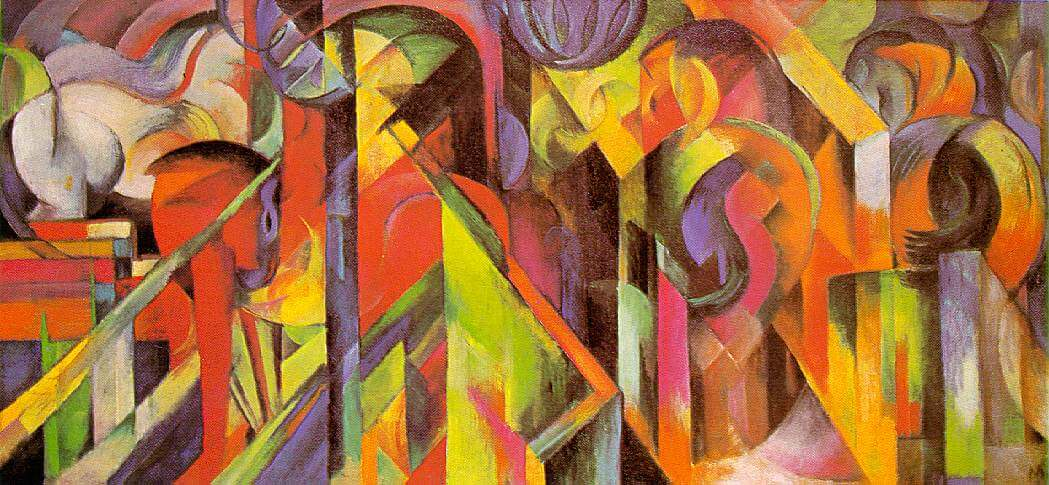
\includegraphics[height=0.4\textwidth]{figures/stables.jpg} % Stables (Stallungen), Franz Marc
\end{figure}

%==============================================================================
\section*{Introduction}

Calculus, broadly speaking, is the study of \textit{rates of change}. That is, calculus is the branch of mathematics required whenever we want to describe a how one quantity changes with respect to another. This makes it of particular importance in physics, which is largely about studying how objects move through space as time advances, but anything that changes over time (like a chemical reaction, an electrical charge, a population, or a stock price) can be studied more closely using calculus.

One of the most important rates of change in physics, and a good place for us to start our introduction to calculus, is \textit{velocity}, the rate of change in an object's position with respect to time. From high school physics you should already be familiar with one type of velocity:~the \textit{average velocity} over some interval of time. For example, if a car is driving along a highway and it crosses mile marker~74 at~2:16pm and then mile marker~106 at~2:41pm, then its average velocity between~2:16pm and~2:41pm is
\begin{align*}
	v_{\text{avg}} &= \frac{\text{change in position between 2:16 and 2:41}}{\text{change in time between 2:16 and 2:41}} = \frac{\text{106 mi $-$ 74 mi}}{\text{41 min $-$ 16 min}} = \frac{\text{32 mi}}{\text{25 min}} = 1.28~\frac{\text{mi}}{\text{min}}
\end{align*}

which is~$76.8$~mph. Average velocity is perfectly easy to define and compute (it's what's called a \textit{difference quotient}, which is exactly what it sounds like), but it doesn't tell us everything about the car's motion. The car's speed probably wasn't exactly~76.8~mph over the entire time interval; it was probably traveling slightly faster at some times and slightly slower at others. Presumably if we had more information (more positions at more times) we would be able to describe the car's \textit{instantaneous velocity}, or its velocity at a specific moment in time.

Instantaneous velocity seems like a simple concept, and in everyday speech we often talk about how fast something is happening ``right now'' or at some other specific moment in time. However, mathematics is all about making vague ideas precise enough to actually use in applications, and it turns out that the notion of instantaneous velocity is surprisingly tricky to define in a sensible, usable way. This worksheet will take you through a sequence of numerical experiments and activities to get you to play around with these ideas for yourself to build up an intuition about how to approach rates of change.

%%%
\subsection*{Required Materials}

This lab includes computational activities in the provided spreadsheet file \verb|rates_of_change.xlsx|. You will need Microsoft Excel\footnote{\url{https://www.microsoft.com/en-us/microsoft-365/excel}} installed in order to access and work with the file. If you cannot access Excel, there are several functionally-equivalent free alternatives that will work just as well (we recommend either Google Sheets\footnote{\url{https://www.google.com/sheets/}} or LibreOffice Calc\footnote{\url{https://www.libreoffice.org/discover/calc/}}).

It is expected that you have some basic familiarity with how to use Excel to perform basic computations, including how to use cell formulas, how to reference other cells, and how to generate plots. If not, the best way to learn is simply to try using it to solve some problems, asking for help from your classmates or the instructor or looking up help online when you get stuck. Using Excel is a skill, and like any skill there is no substitute for practice.

%%%
\subsection*{Learning Objectives}

After completing this project, you should be able to:
\begin{itemize}
	\item Explain how the idea of an instantaneous rate of change is related to average rates of change.
	\item Use a computer to help to answer questions about a function's rate of change, like when its value is increasing/decreasing/constant and when it is changing the fastest.
	\item Work with a real-world function defined as a table of values rather than as a simple formula.
	\item Be comfortable using a computer alongside analytical work by hand in order to solve a complicated problem.
\end{itemize}

%==============================================================================

% Instantaneous Velocity of a Weather Balloon
\newpage
%\section{Instantaneous Velocity of a Weather Balloon}
\section*{Instantaneous Velocity of a Weather Balloon}
\label{sec:balloon}

As noted above, average velocity is easy to compute, but we don't yet have a way to approach computing instantaneous velocities. In this activity you will work with a (lightly edited) set of position data gathered from a weather balloon launched from the Salton Sea weather station on February~28,~2021\footnote{F.~M.~Ralph, A.~M.~Wilson, R.~Demirdjian, D.~Alden, C.~Hecht, C.~J.~Ellis, B.~Kawzenuk, F.~Cannon, A.~Cooper, and K.~Paulsson. Radiosonde Data Collected During California Storms. UC~San~Diego Library Digital Collections, Dataset, 2021. \href{https://doi.org/10.6075/J09P31S0}{doi:10.6075/J09P31S0}} to try to see how we might approach the problem of how to describe the balloon's instantaneous velocity.

%%%
\subsection*{Activity}

%\begin{enumerate}[\bf {\thesection}a.]
\begin{enumerate}
	\item Open the activity spreadsheet \verb|rates_of_change.xlsx| and make sure that you're on the first tab, labeled ``Weather Balloon''. You should see two very long columns of data:~column~\textbf{A} indicates the time~(in~seconds since the launch) and column~\textbf{B} indicates the position~(in~meters north of the launch site) of the balloon\footnote{Only the balloon's position in the longitudinal direction is included here. The original data set included latitudes and altitudes, but for this activity we're going to pretend that all of its motion occurs in a single direction. Describing movement through~3D space is a significantly more complicated topic covered in Calculus~III (Multivariate~Calculus).}. The data series includes~5409 times in~1-second increments spanning a period of just over~1.5~hours.
	
	\item Shortly we will be computing some velocity measurements for the balloon, but before that we can at least try to come up with some preliminary results using our eyes. Create a scatter plot of the balloon's position versus time, and use the graph to estimate the following:
	\begin{itemize}
		\item Over what time interval was the balloon moving north? South?
		\item Are there any times at which the balloon stopped moving momentarily?
		\item At what time was the balloon moving the fastest?
	\end{itemize}
	
	Explain the reasoning behind each of your guesses.
	
	\item Over the next few parts we will attempt to answer one fundamental question:~What was the \textit{instantaneous} velocity of the balloon at time~60~seconds? We will work our way up to that answer by starting with a few smaller, simpler numerical experiments.
	
	It's not immediately obvious how to compute an instantaneous velocity, but we know exactly how to compute an \textit{average} velocity, so that might be a good place to start. At least intuitively we might expect the instantaneous velocity at~60~seconds to be similar to the average velocities over time intervals that are ``close~to''~60.
	
	Compute the average velocity of the balloon over the time interval from~60 to~70 seconds. Then try it from~60 to~65 seconds, then from~60 to~61 seconds. What are the units of the values you've just computed? If you had to choose one of them as your ``best guess'' for the instantaneous velocity at time~60, which would you pick? Why do you think your choice is more reasonable than the others?
	
	\item We can use Excel to quickly automate this process to compute many different average velocities over many different time intervals. Use column~\textbf{C} to compute the average velocity between \textit{every} time and time~60. For example, the entry in the row for time~16 should compute the average velocity between~60 and~16 seconds, the entry in the row for time~763 should compute the average velocity between~60 and~763, and so on\footnote{Hint:~In Excel, a dollar sign~(\texttt{\$}) can be used to keep part of a cell reference constant within a formula as it is copied into other cells. In this case each average velocity computation needs to reference cells in two different rows, one of which should remain constant (the reference for time~60) and one of which should not (the reference for the other time's row).}.
	
	\item Create a scatter plot of these average velocities versus time. You should see what appears to be a relatively normal, well-behaved, continuous-looking function.
	
	It's hard to see what's happening around time~60 in this graph due to the scale. Try plotting the average velocities again, this time only including times between~50 and~70~seconds. What happens to the graph immediately around~60~seconds? What happens to it exactly at~60 seconds?
	
	\item We started looking at average velocities based on the idea that an average velocity over an interval ``close~to''~60 should give us some idea of the instantaneous velocity there. Look up the average velocity that your Excel formula actually computed at time~60. Why has it resulted in an error?
	
	\item Based on the previous experiments, apparently it's not possible for us to compute an instantaneous velocity at a time by just computing an average velocity over a time interval of zero width. Since the weather balloon's position is given to us as a set of finitely-many discrete values there is a smallest nonzero time interval that we can consider (1~second). In class we will see how all of this changes for a \textit{continuous} position function, but for now let's continue to work with the idea that we can at least \textit{approximate} an instantaneous velocity at a time by using an average velocity over a small time span around that time.
	
	Apply this idea to compute an instantaneous velocity estimate for \textit{every} time in column~\textbf{D}. For example, the entry in the row for time~16 should compute an approximation for the instantaneous velocity at time~16, the entry in the row for time~763 should compute an approximation for the instantaneous velocity at time~763, and so on\footnote{Hint:~Most of the cells can be handled with a single formula copied into every row, but the first and last rows may need to be handled separately, since any average velocity computed for the first time cannot include data from an earlier time, and any average velocity computed for the last time cannot include data from a later time.}.
	
	\item Create a scatter plot of these (approximate) instantaneous velocities versus time. You should see a somewhat jagged but still relatively well-behaved and continuous-looking graph. Use the velocity graph to estimate the following:
	\begin{itemize}
		\item Over what time interval was the balloon moving north? South?
		\item Are there any times at which the balloon stopped moving momentarily?
		\item At what time was the balloon moving the fastest?
		\item Now that you actually have a velocity graph you can answer a more precise follow-up question:~What was the balloon's maximum velocity?
	\end{itemize}
	
	Explain the reasoning behind each of your guesses.
	
	\item Finally, look at your velocity graph alongside your original position graph. What is happening to the shape of the position graph where the velocity graph crosses the $x$-axis? When it's positive? When it's negative?
\end{enumerate}


\end{document}
